\documentclass{article}

% Packages
\usepackage{graphicx} % required for inserting images
\usepackage{geometry}
\usepackage{amssymb}
\usepackage{amsmath}
\usepackage{comment}
\usepackage{mathtools, nccmath}

\newgeometry{vmargin={15mm}, hmargin={20mm}}
\title{EECS 199 - Pump and PH Testing System}
\author{Ivan Tran}
\date{}
\begin{document}
    \maketitle

    \section{Overview}
        \begin{flushleft}
            This report will detail the systems that we used to conduct the pump and pH testing experiments.
            \begin{itemize}
                \item \textbf{Pump Testing}: For the pump experiment, we tested the rate that volume was dispensed to see if it matches the product specification.
                \item \textbf{pH Testing}: For the pH experiment, we calibrated the pH module to see if it measured pH accurately. We then tested how the pH probe reading would change as we added acid and base solutions.
            \end{itemize}
        \end{flushleft}

    \section{Hardware}
        \subsection{Pump Circuit}
            \begin{flushleft}
                A schematic for the pump circuit is shown in the image below:
                \begin{figure}[!hbt]
                    \centering
                    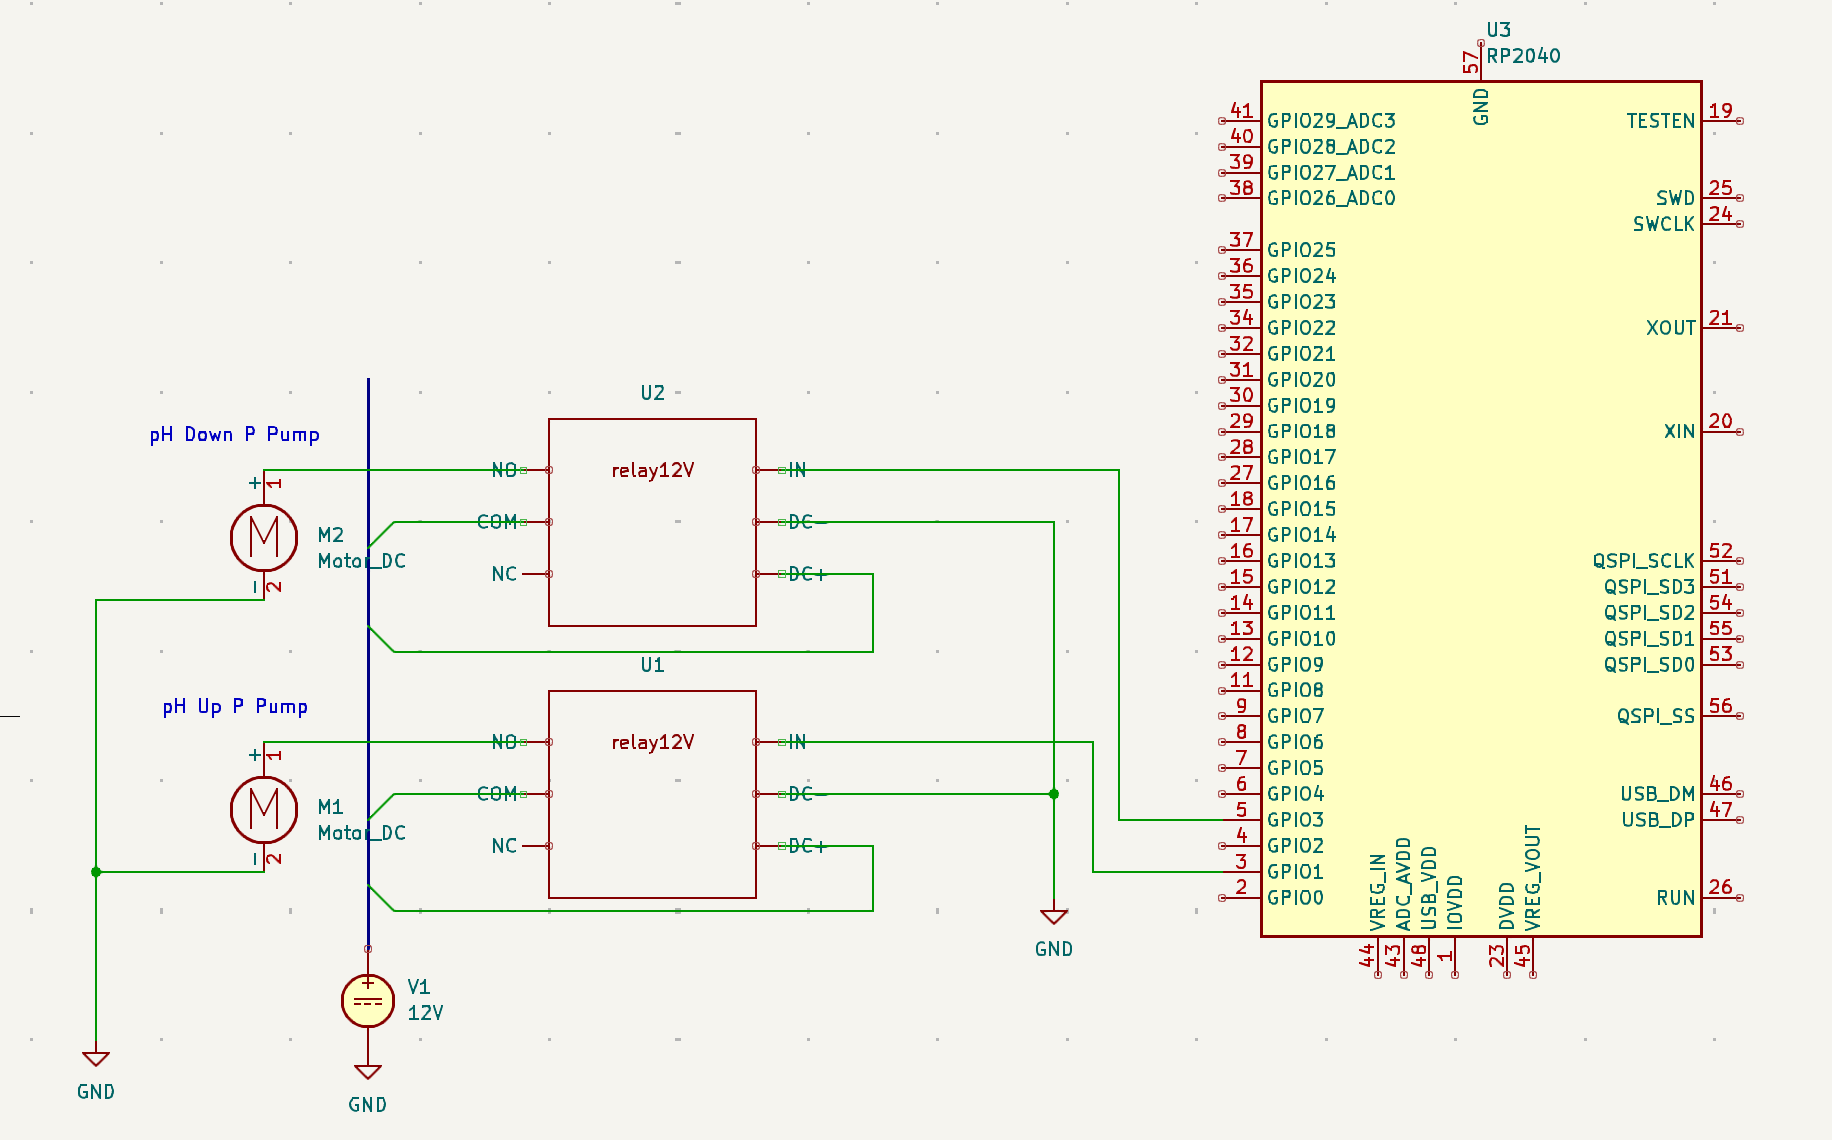
\includegraphics[width=0.50\linewidth]{assets/pumpCircuitSchematic.png} % paste image w/i these brackets
                \end{figure}
            \end{flushleft}
        \subsection{pH Testing Circuit}
            \begin{flushleft}
                A schematic for the pH Testing circuit is shown below
            \end{flushleft}
\end{document}
